\section{Value Proposition and Business Model}
The hypothethis is made that the customers and the users of this product are different. Indeed the people buying the device will be the family of the elder(s). While the elders will be the end users. Therefore the needs of the buyers and of the users are different. They will be both be using the device but through two different interfaces.

The value proposion canvas template used for the analysis is the one pictured in Figure~\ref{}.

begin{figure}[!htb]
    \centering
    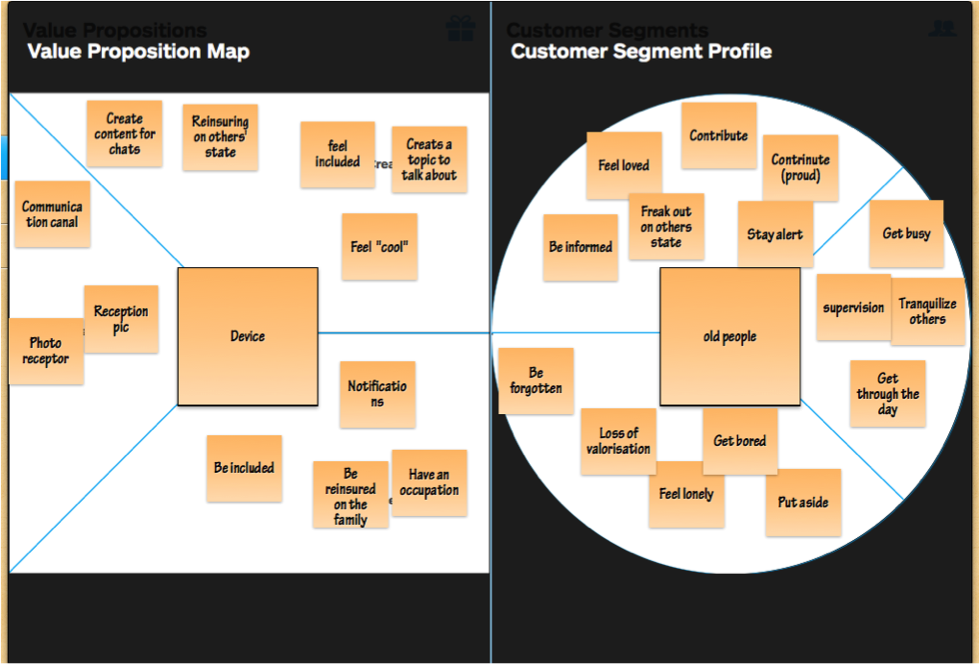
\includegraphics[width=0.9\textwidth,keepaspectratio]{chap/marketFig/elderly_value_prop_canvas.png}
    \caption{Business model canvas}
    \label{fig:elders value proposition}
\end{figure}

\subsection{Value Proposition}
As the customers and the users are not the same people we made two value proposition canvases.
The value propostion canvas for the elderly can be seen in figure \ref{fig:value proposition}.

\begin{figure}[!htb]
    \centering
    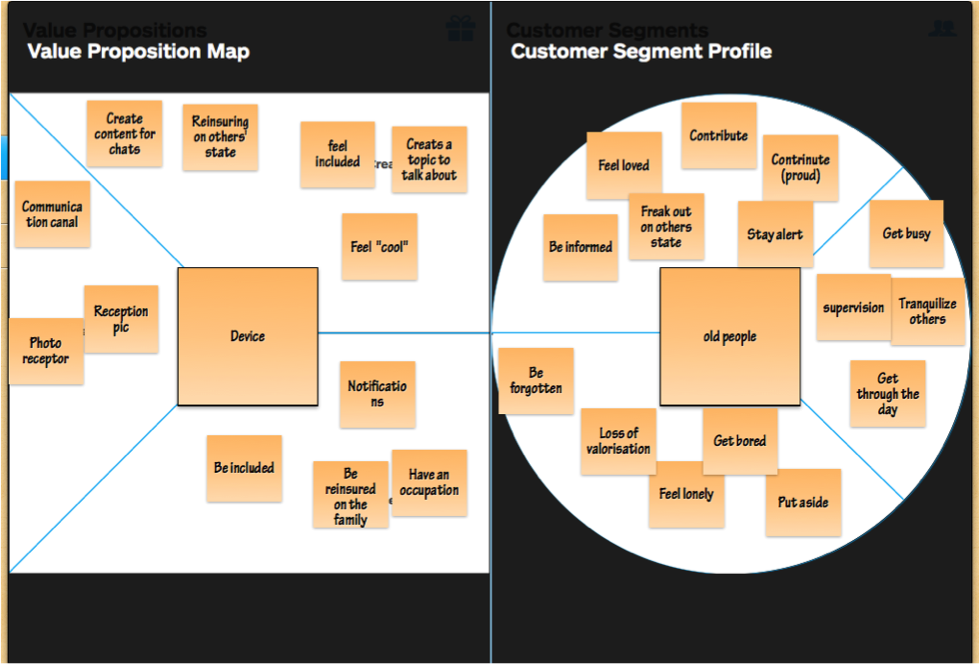
\includegraphics[width=0.9\textwidth,keepaspectratio]{chap/marketFig/elderly_value_prop_canvas.png}
    \caption{Business model canvas}
    \label{fig:elders value proposition}
\end{figure}

\subsection{business model}

The business model canvas is shown in the figure \ref{fig:business model}.

\begin{figure}[!htb]
    \centering
    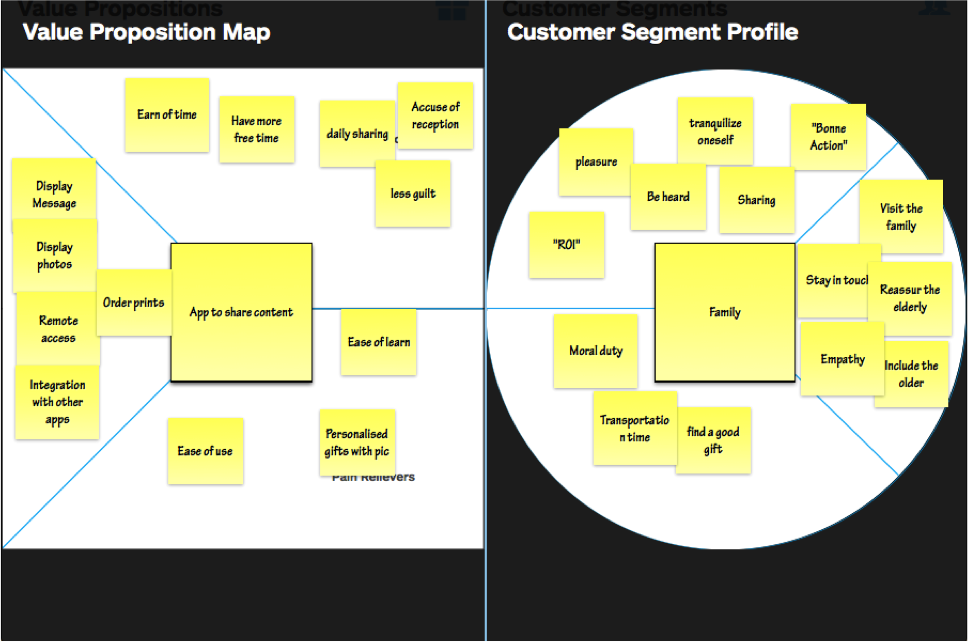
\includegraphics[width=0.9\textwidth,keepaspectratio]{chap/marketFig/family_value_prop_canvas.png}
    \caption{business model canvas}
    \label{fig:business model}
\end{figure}

\subsection{User tests}
